\chapter{Docker}
Docker \cite{docker} is a set of PaaS products that uses OS virtualization to deliver software in packeges called containers. A container is a unit of software that packages up software and its dependencies, so the application runs and could also be shared. 
\\\\
To develop a docker container there are several options: one is to create a Docekerfile in which we can detail all the specifications and the features that we want to run in that container. Usually that is to run a single application in a sandbox environment.  
\\
In the study case the application is an OpenLDAP server. To run that it’s needed an operating system: the choice i made is to use a debian image.
\section{Creation of the container}
\begin{mdframed}[backgroundcolor=back]
\lstinputlisting[style=docker]{code/Dockerfile}
\end{mdframed}
Once the base image is chosen, it is necessary to install the package that will be used. The list of packages is shown in the figure. In particular slapd is the daemon that runs the ldap server, ldap-utils contains all the tools to search, add, modify and delete entries from the server from the outside. The others contains usefull tools that will be used in the next steps.  
\\
After that it is made a copy of the deception and configuration data inside the conteiner, and are exposed two ports for reach the container from the outside. Two ports because one is for the base TCP connection (10389) and one for the connection using TLS (10636). 
\\
At the end of the Dockerfile it’s launched a script that configures the server.
\section{Configuration scripts}
The scripts are writen in bash and call, starts and configure the daemon used in the data generation and the one that starts the server. In particular:
\begin{itemize}
    \item one is used to reconfigure the server
    \item the other is used to run the server using the specified ports
    \item the last is used tu activare all the required components
\end{itemize}
\\
In the first scripts are present four functions:\\
\begin{itemize}
    \item \textit{reconfigure\_slapd()}
    \item \textit{configure\_admin\_conig\_pw()}
    \item \textit{load\_initial\_data()}
    \item \textit{convert\_schema()}
\end{itemize}
\\
The first one configures the server using the info submitted in the Dockerfile. This step is needed because when slapd is installed it creates a default config, so to modify the dafault paramenters we use that function.
\\
The \textit{configure\_admin\_config\_pw()} insert the info of a specific ldif file that contains data about the adimn.
\\
\textit{load\_initial\_data()} finds all the ldif files inserted into the copied folder and add them following a specified order (in our case the order is taken from the file names).
\\
The last function converts the .schema files into .ldif definitions, using the tool \textbf{schema2ldif} \cite{schema2ldif} and add them into the directory.
\\
After that configuration steps the server is created. To allow it to run on the exposed ports, it's stopped and reactivated using the following script.
\begin{mdframed}[backgroundcolor=back]
\lstinputlisting[style=bash]{code/slapd-init.sh}
\end{mdframed}
Once generated the Dockerfile and the relative configuration we can run the container and see that it works.
\begin{figure}[h]
    \caption{Example of working container}
    \centering
    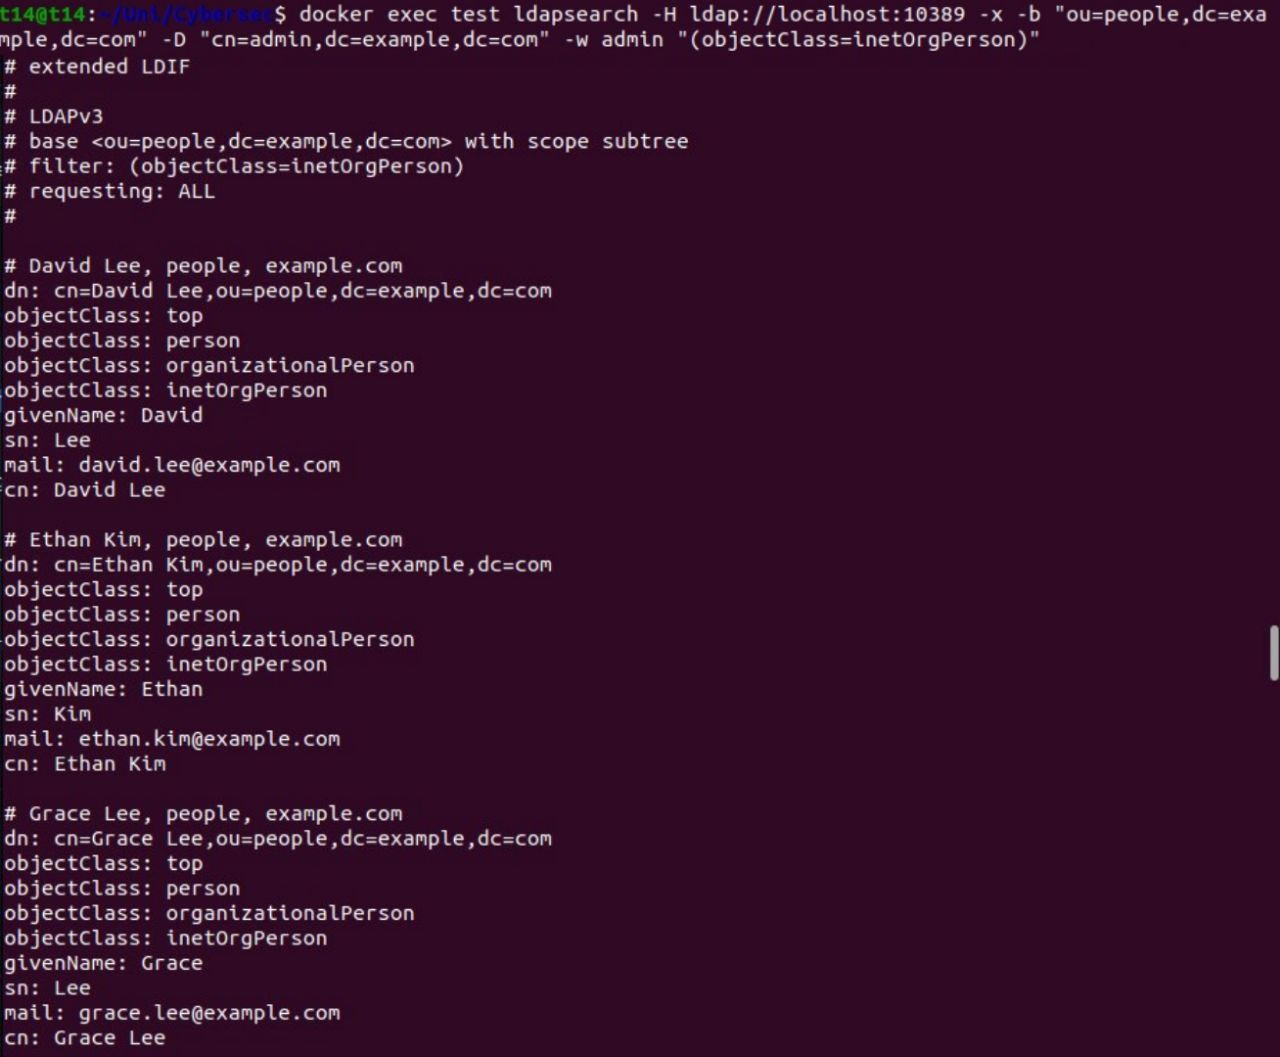
\includegraphics[width=10cm]{img/search.jpg}
\end{figure}
